\section{Application: Sketching}
\label{appendix:sketching}
Beyond random projection, our novel TRP also has an important application in sketching. Sketching is an important technique to accelerate expensive computations with widespread applications, such as regression, low-rank approximation, and graph sparsification, etc. \citep{halko2011finding,woodruff2014sketching} 
% I have to think about how to argue tensor has a natural Khatri-Rao structure. 
The core idea behind sketching is to compress a large dataset, typically a matrix or tensor, into a smaller one by multiplying a random matrix. 
%Since the matrix multiplication is a linear operation, people can usually further extend sketching to distributed and online setting. 
In this section, we will mainly focus on the low-rank matrix approximation problem. Consider a matrix $\mathbf{X} \in \mathbb{R}^{m \times d}$ with rank $r$, 
we want to find the best rank-$r$ approximation with the minimal amount of time. The most common method is the randomized singular value decomposition (SVD), whose underlying idea is sketching. 


First, we compute the linear sketch $\mathbf{Z} \in \mathbb{R}^{m \times k}$ by $\mathbf{Z} =\mathbf{X}\mathbf{\Omega}$, where $\mathbf{\Omega} \in \mathbb{R}^{d \times r}$ is the random map. Then we compute the QR decomposition of $\mathbf{X}\mathbf{\Omega}$ by $\mathbf{Q}\mathbf{R} = \mathbf{Z}$, where $\mathbf{Q} \in \mathbb{R}^{m \times k}, \mathbf{R} \in \mathbb{R}^{r \times r}$. At the end, we project $\mathbf{X}$ onto the column space of $\mathbf{Q}$, and obtain the approximation $\hat{\mathbf{X}} = \mathbf{Q} \mathbf{Q}^\top \mathbf{X}$.  

With our TRP, we can significantly reduce the storage of the random map, while achieving similar rate of convergence as demonstrated in Figure \ref{fig:col_matrix}. 
With further variance reduction by taking the geometric-median over multiple runs, our TRP with variance reduction can achieve even better performance. The detailed implementation is given in Algorithm \ref{alg:var-red-structure-sketching}. And we will delay the theoretical analysis of this method for future works. 


\begin{algorithm}[H]
	\caption{Tensor Sketching with Variance Reduction}\label{alg:var-red-structure-sketching}
	\begin{algorithmic}[1]
		\Require $\mathbf{X} \in \mathbb{R}^{m \times d}$, where $d = \prod_{i=1}^N d_n$ and 
		\rm{RMAP} is a user-specified function that generates a random dimension reduction map. $T$ is the number of runs for variance reduction averaging. 
		\Function{SSVR}{$\mathbf{X}, \{d_n\}, k, T, \rm{RMAP}$}\\
		\text{For $t= 1 \dots T$}\\
		\text{For $i = 1 \dots N$} \\
		$\mathbf{\Omega}_i^{(t)} = \rm{RMAP}(d_i, k)$
		\State $\mathbf{\Omega}^{(t)} = \mathbf{\Omega}_1^{(t)} \odot \cdots \odot \mathbf{\Omega}_{N}^{(t)}$
		\State $(\mathbf{Q}^{(t)}, \sim ) = \rm{QR}(\mathbf{X}\mathbf{\Omega}^{(t)})$ 
		\State $\hat{\mathbf{X}}^{(t)} = \mathbf{Q}^{(t)}\mathbf{Q}^{(t)T}\mathbf{X}$
		\State
		$\hat{\mathbf{X}} = \frac{1}{T}\sum_{t=1}^T \hat{\mathbf{X}}^{(t)}$
		\State \Return $\mathbf{G}$
		\EndFunction
	\end{algorithmic}
\end{algorithm}

Furthermore, the extension of TRP to tensor data is also natural. To be specific, the $n^{th}$ unfolding of a large tensor $\mathscr{X} \in \mathbb{R}^{I_1 \times \cdots \times I_N}$, denoted as $\mathbf{X}^{(n)}$, has dimension $I_n \times I_{(-n)}$, where $I_{(-n)} = \prod_{i \neq n, i \in [N]} I_i$ . To construct a sketch for the unfolding, we need to create a random matrix of size $ I_{(-n)} \times k$. Then, our TRP becomes a natural choice to avoid the otherwise extremely expensive storage cost. For many popular tensor approximation algorithms, it is even necessary to perform sketching for every dimension of the tensor \citep{de2000multilinear,wang2015fast}. 
%such as Higher-Order Orthogonal Iteration \citep{de2000multilinear}, Fast CANDECOMP/PARAFAC decomposition \citep{wang2015fast}, our paper ? 
In the simulation section, we perform experiments for the unfolding of the higher-order order tensor with our structured sketching algorithms (Figure \ref{fig:col_matrix}). For more details in tensor algebra, please refer to \citep{kolda2009tensor}. 


\paragraph{Experimental Setup}
In sketching problems, considering a $N$-D tensor $\mathscr{X} \in \mathbb{R}^{I^N}$ with equal length along all dimensions, we want to compare the performance of the low rank approximation with different maps for its first unfolding $\mathbf{X}^{(1)} \in \mathbb{R}^{I \times I^{N-1}}$. 
	
We construct the tensor $\mathscr{X}$ in the following way. Generate a core tensor $\mathscr{C} \in \mathbb{R}^{r^N}$, with each entry $\rm{Unif}([0,1])$. Independently generate $N$ orthogonal arm matrices by first creating $\mathbf{A}_1, \dots, \mathbf{A}_N \in \mathbb{R}^{r \times I}$ and then computing the arm matrices by $(\mathbf{Q}_n, \sim) = \rm{QR}(\mathbf{A}_n)$, for $1 \leq n \leq N$.
\begin{equation}
\mathscr{X} = \mathscr{C} \times_1 \mathbf{Q}_1 \cdots \times_N \mathbf{Q}_N + \sqrt{\frac{0.01 \cdot \|\mathscr{X}^\natural\|_F^2}{I^N}} \mathcal{N}(0,1). \nonumber
\end{equation}
Then, we construct the mode-1 unfolding of $\mathbf{X} = \mathbf{X}^{(1)}$, which has a rank smaller than or equal to $r$. 

In our simulation, we consider the scenarios of 2-D ($900 \times 900$), 3-D ($400 \times 400 \times 400$), 4-D ($100 \times 100 \times 100 \times 100$) tensor data, with corresponding mode-1 unfolding of size $900 \times 900$, $400 \times 160000$, $100 \times 1000000$ respectively and $r = 5$. In each scenario, we compare the performance for Gaussian RP, TRP, and $\textup{TRP}_5$ maps with varying $k$ from 5 to 25. The TRP map in these scenarios has 2, 4, 6 components of size $30 \times k$, $20 \times k$, $10 \times k$ respectively. And the number of runs variance reduction averaging is $T = 5$. In the end, we evaluate the performance by generating the random matrix 100 times and compute the relative error $\frac{\|\mathbf{X} - \hat{\mathbf{X}}\|}{\|\mathbf{X}\|}$, and constructing a 95\% confidence interval for it.

\paragraph{Result}From Figure \ref{fig:col_matrix}, we can observe that the relative error decreases as $k$ increases as expected for all dimension reduction maps. The difference of the performance between the Khatri-Rao map and Gaussian map is small when $N = 2$, but increases when $N$ increases, whereas the Khatri-Rao variance reduced method is particularly effective producing strictly better performance than the other two. 

\begin{figure*}[ht!]
	\centering
	\begin{subfigure}{0.32\textwidth}
		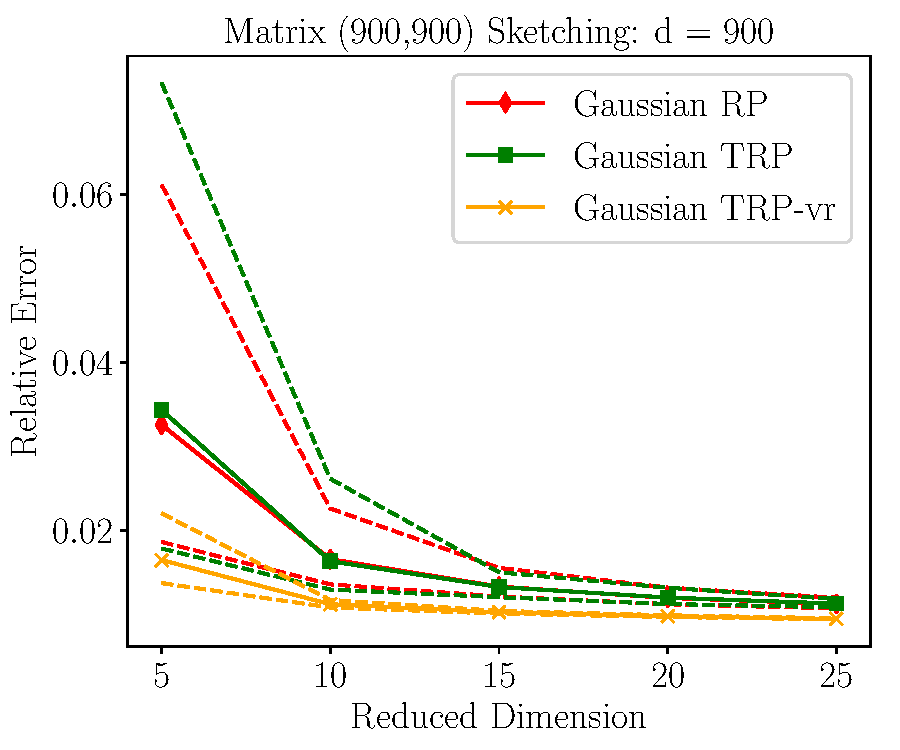
\includegraphics[scale = 0.3]{figure/col_dim2_krao_d900.pdf}
	\end{subfigure}
	\begin{subfigure}{0.32\textwidth}
		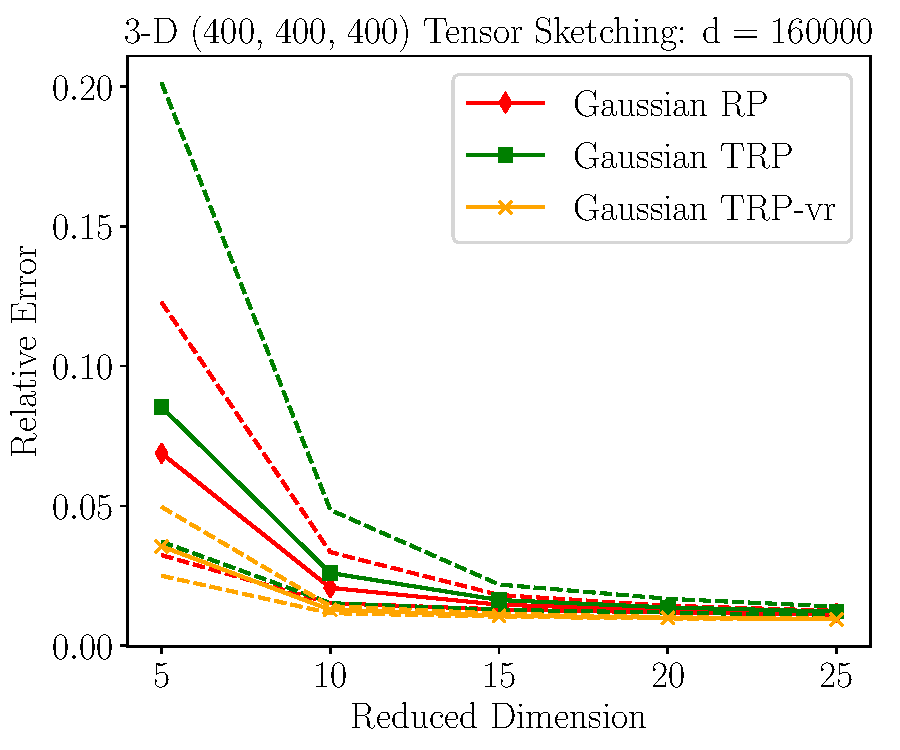
\includegraphics[scale = 0.3]{figure/col_dim3_krao_d160000.pdf}
	\end{subfigure}
	\begin{subfigure}{0.32\textwidth}
		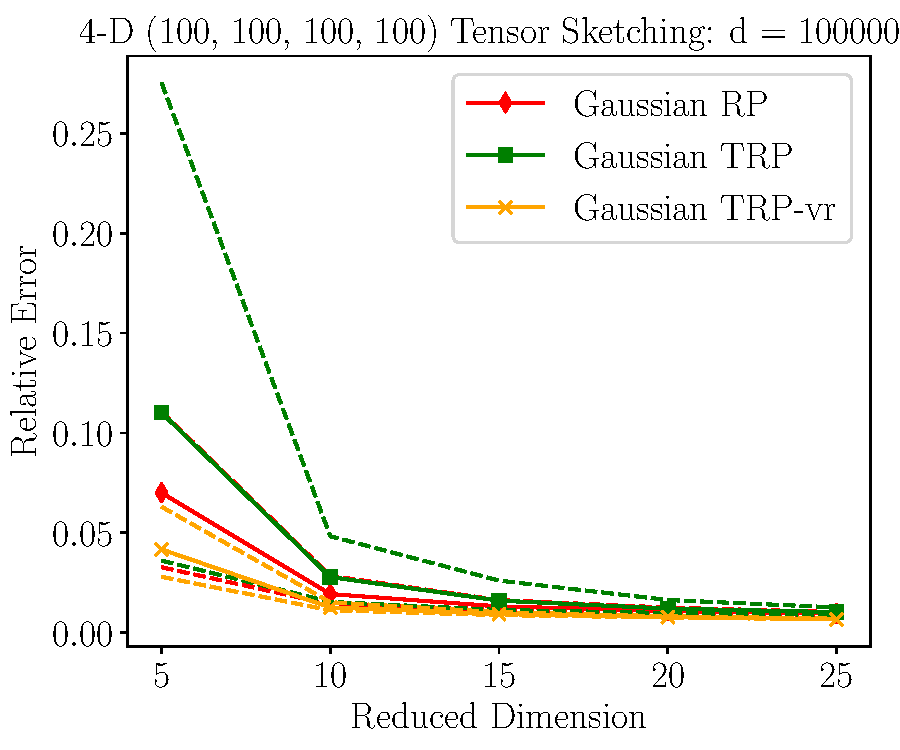
\includegraphics[scale = 0.3]{figure/col_dim4_krao_d1000000.pdf}
	\end{subfigure}\\
	\caption{Relative Error for the low-rank tensor unfolding approximation: \textit{we compare the relative errors for low-rank tensor approximation with different input size: 2-D ($900 \times 900$), 3-D ($400 \times 400 \times 400$), 4-D ($100 \times 100 \times 100 \times 100$). In each setting, we compare the performance of Gaussian RP, TRP, and $\textup{TRP}_5$. The dashed line stands for the 95\% confidence interval.}}
	\label{fig:col_matrix}
\end{figure*}

